\subsection{\texorpdfstring{\(W_{n}(A)\) 的有限长度 Witt 向量环}{W\_\{n\}(A) 的有限长度 Witt 向量环}}

定义 2．——设 A 为一个环，\(n \geqslant 1\) 为整数。记 \(\mathbf{W}_{n}(\mathbf{A})\) 为商环 \(\mathbf{W}(\mathbf{A}) / \mathbf{V}_{n}(\mathbf{A})\)。

给定 A 中的元素 \(a_0, \ldots, a_{n-1}\)，将类 \([a_0, \ldots, a_{n-1}]\) 或 \([a_i]_{0 \leq i < n}\) 记作 \(\mathrm{V}_n(\mathrm{A})\) 模元素 \((a_0, \ldots, a_{n-1}, 0, 0, \ldots)\)（属于 \(\mathrm{W}(\mathrm{A})\)）的类。根据第 6 节引理 4，映射 \((a_0, \ldots, a_{n-1}) \mapsto [a_0, \ldots, a_{n-1}]\)（从 \(\mathrm{A}^n\) 到 \(\mathrm{W}_n(\mathrm{A})\)）是双射。因此，称 \(\mathrm{W}_n(\mathrm{A})\) 的元素为长度为 \(n\) 的 Witt 向量；类比地，\(\mathrm{W}(\mathrm{A})\) 的元素

有时也称为无限长度的 Witt 向量。记 \(\pi_n\) 为从 W(A) 到 \(\mathrm{W}_n(\mathrm{A})\) 的典范同态。根据第 6 节引理 4，有

\[
\pi_ {n} (\boldsymbol {a}) = [ a _ {0}, \dots , a _ {n - 1} ]\tag{42}
\]

对 W(A) 中的每个 \(\boldsymbol{a} = (a_{n})_{n \in \mathbb{N}}\) 均成立。

根据 W(A) 中运算的定义，\(\mathrm{W}_{n}(\mathrm{A})\) 中的运算可如下描述：

\[
\begin{array}{r l} & {[ a _ {0},..., a _ {n - 1} ] + [ b _ {0},..., b _ {n - 1} ] = [ \mathrm{S} _ {i} (a _ {0},..., a _ {i}; b _ {0},..., b _ {i}) ] _ {0 \leqslant i <   n}} \\ & {[ a _ {0},..., a _ {n - 1} ] \times [ b _ {0},..., b _ {n - 1} ] = [ \mathrm{P} _ {i} (a _ {0},..., a _ {i}; b _ {0},..., b _ {i}) ] _ {0 \leqslant i <   n}} \\ & {\quad - [ a _ {0},..., a _ {n - 1} ] = [ \mathrm{I} _ {i} (a _ {0},..., a _ {i}) ] _ {0 \leqslant i <   n}.} \end{array}
\]

此外，\(\mathbf{W}_{n}(\mathbf{A})\) 中的加法单位元是 \([0,\dots,0]\)，乘法单位元是 \([1,0,\dots,0]\)。

设 \(i\) 为满足 \(0 \leqslant i \leqslant n\) 的整数。通过取商，从 W(A) 到 A 的同态 \(\Phi_{i}\) 定义了同态 \(\Phi_{i}\)，它从 W \(_{n}\) (A) 到 A。此映射将 Witt 向量 \([a_{0}, ..., a_{n-1}]\) 关联到 A 中的元素 \(\Phi_{i}(a_{0}, ..., a_{i})\)（也称为下标为 \(i\) 的 \([a_{0}, ..., a_{n-1}]\) 的幽灵分量）。

设 \(\rho : \mathbf{B} \to \mathbf{A}\) 为一个环同态。通过取商，同态 \(\mathbf{W}(\rho)\)（从 \(\mathbf{W}(\mathbf{B})\) 到 \(\mathbf{W}(\mathbf{A})\)）定义了同态 \(\mathbf{W}_n(\rho)\)，后者从 \(\mathbf{W}_n(\mathbf{B})\) 到 \(\mathbf{W}_n(\mathbf{A})\)。它由公式

\[
\mathrm{W} _ {n} (\rho) \left[ b _ {0},..., b _ {n - 1} \right] = \left[ \rho (b _ {0}),..., \rho (b _ {n - 1}) \right]\tag{43}
\]

对每个 \([b_0, \ldots, b_{n-1}]\)，只要它属于 \(\mathbf{W}_n(\mathbf{B})\)，均成立。

设 \(m\)、\(n\) 为满足 \(1 \leqslant n \leqslant m\) 的两个整数。由于 \(V_n(A) \supset V_m(A)\)，存在从 \(W_m(A) = W(A)/V_m(A)\) 到 \(W_n(A) = W(A)/V_n(A)\) 的典范满射同态；将此同态记为 \(\pi_{n,m}\)。明确地说，有

\[
\pi_ {n, m} [ a _ {0}, \dots , a _ {m - 1} ] = [ a _ {0}, \dots , a _ {n - 1} ]\tag{44}
\]

对每个 \([a_0, \ldots, a_{m-1}]\)，若它属于 \(\mathrm{W}_m(\mathrm{A})\)，上述结论均成立。族 \((\mathrm{W}_n(\mathrm{A}), \pi_{n,m})\) 是一个环的逆系统，而映射 \(\pi: \boldsymbol{a} \mapsto (\pi_n(\boldsymbol{a}))_{n \geqslant 1}\) 是从 \(\mathrm{W}(\mathrm{A})\) 到 \(\lim \mathrm{W}_n(\mathrm{A})\) 的环同态，称为典范同态。由于 \(\mathrm{W}(\mathrm{A})\) 关于滤子 \((\overleftarrow{\mathrm{V}_n(\mathrm{A})})_{n \in \mathbb{Z}}\) 是分离且完备的（参见第 6 节），典范同态 \(\pi\) 是拓扑环同构，其中给 \(\mathrm{W}_n(\mathrm{A})\) 赋予离散拓扑，且 \(n \geqslant 1\) 遍历所有整数（III，第 2 节第 6 号）。

从现在起，分别将同态 \(\pi_{n}\) 和 \(\pi_{n,m}\) 称为从 W(A) 到 \(\mathrm{W}_{n}(\mathrm{A})\) 以及从 \(\mathrm{W}_{m}(\mathrm{A})\) 到 \(\mathrm{W}_{n}(\mathrm{A})\) 的投影同态。

例．——1) 同态 \(\Phi_{0}:W_{1}(A)\to A\) 是同构。

\begin{enumerate}
\def\labelenumi{\arabic{enumi})}
\setcounter{enumi}{1}
\tightlist
\item
  具体写出 \(W_{2}(A)\) 中的运算。我们有
\end{enumerate}

\[
\begin{array}{l} \left[ a _ {0}, a _ {1} \right] + \left[ b _ {0}, b _ {1} \right] = \left[ a _ {0} + b _ {0}, a _ {1} + b _ {1} - \sum_ {i = 1} ^ {p - 1} \frac {1}{p} \binom {p} {i} a _ {0} ^ {i} b _ {0} ^ {p - i} \right] \\ \left[ a _ {0}, a _ {1} \right] \times \left[ b _ {0}, b _ {1} \right] = \left[ a _ {0} b _ {0}, a _ {0} ^ {p} b _ {1} + a _ {1} b _ {0} ^ {p} + p. a _ {1} b _ {1} \right] \end{array}
\]

对于 \([a_0, a_1]\) 和 \([b_0, b_1]\)，它们属于 \(\mathbf{W}_2(\mathbf{A})\)，\([a_0, a_1]\) 的幽灵分量为 \(a_0\) 和 \(a_0^p + p \cdot a_1\)。

\begin{enumerate}
\def\labelenumi{\arabic{enumi})}
\setcounter{enumi}{2}
\tightlist
\item
  设 \(n \geqslant 1\) 为整数。若 \(a_0, \ldots, a_{n-1}, b_0, \ldots, b_{n-1}\) 是满足 \(a_i \equiv b_i \mod p\)（\(0 \leqslant i < n\)）的整数，则有（第 1 节命题 1）
\end{enumerate}

\[
\Phi_ {n - 1} (a _ {0}, \dots , a _ {n - 1}) \equiv \Phi_ {n - 1} (b _ {0}, \dots , b _ {n - 1}) \bmod p ^ {n}.
\]

因此，通过取商，\(\Phi_{n-1}\) 定义了环同态 \(\varphi_n: \mathrm{W}_n(\mathbf{Z}/p\mathbf{Z}) \to \mathbf{Z}/p^n\mathbf{Z}\)。\(\varphi_n\) 的像是包含 1 的 \(\mathbf{Z}/p^n\mathbf{Z}\) 的子群，故 \(\varphi_n\) 是满射。由于有限集 \(\mathrm{W}_n(\mathbf{Z}/p\mathbf{Z})\) 和 \(\mathbf{Z}/p^n\mathbf{Z}\) 的基数同为 \(p^n\)，\(\varphi_n\) 是同构。

设 \(m\)、\(n\) 为满足 \(1 \leqslant n \leqslant m\) 的整数。存在唯一的环同态 \(\alpha_{n,m} : \mathbf{Z}/p^{m}\mathbf{Z} \to \mathbf{Z}/p^{n}\mathbf{Z}\)；因而下图

\pandocbounded{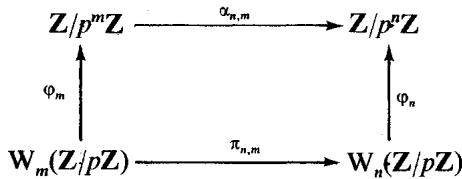
\includegraphics[keepaspectratio]{images/part001_40a15710.jpg}}

是交换的。由此，\(\varphi = \varprojlim \varphi_n\) 是从 \(\mathbf{W}(\mathbf{Z}/p\mathbf{Z}) = \varprojlim \mathbf{W}_n(\mathbf{Z}/p\mathbf{Z})\) 到 \(\mathbf{Z}_p = \varprojlim \mathbf{Z}/p^n\mathbf{Z}\) 的拓扑环同构（III，第 2 节第 12 号例 3）。

设 \(m\)、\(n\) 为两个 \(\geqslant 1\) 的整数。按构造，有加法群的正合序列

\[
0 \longrightarrow \mathrm{W} (\mathrm{A}) \xrightarrow {\mathrm{V} ^ {m}} \mathrm{W} (\mathrm{A}) \xrightarrow {\pi_ {m}} \mathrm{W} _ {m} (\mathrm{A}) \longrightarrow 0.\tag{E}
\]

通过取商，W(A) 的加法群自同态 \(V^{n}\) 定义了同态 \(V_{m}^{n}\)，其从 \(W_{m}(A)\) 的加法群到 \(W_{m+n}(A)\) 的加法群。换言之，有交换图

\pandocbounded{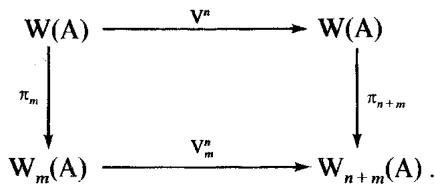
\includegraphics[keepaspectratio]{images/part001_7fe9268c.jpg}}

通过取商，由正合序列 (E) 得到正合序列

\[
0 \longrightarrow \mathrm{W} _ {m} (\mathrm{A}) \xrightarrow {\mathrm{V} _ {m} ^ {n}} \mathrm{W} _ {n + m} (\mathrm{A}) \xrightarrow {\pi_ {n , n + m}} \mathrm{W} _ {n} (\mathrm{A}) \longrightarrow 0.\tag{E'}
\]

有

\[
\mathrm{V} _ {m} ^ {n} [ a _ {0}, \dots , a _ {m - 1} ] = [ \underbrace {0 , \dots , 0} _ {n \text {   times }}, a _ {0}, \dots , a _ {m - 1} ],\tag{45}
\]

对每个元素 \([a_0, \ldots, a_{m-1}]\)，只要它属于 \(\mathbf{W}_m(\mathbf{A})\)，均成立。

根据第 5 节命题 3 的 c)，对 W(A) 中的所有 a，有 FV \(^{m+1}\) (a) = p.V \(^{m}\) (a)，从而 F(V \(_{m+1}\) (A)) ⊂ V \(_{m}\) (A)。对 n 归纳可知，F \(^{n}\) 将 V \(_{n+m}\) (A) 映入 V \(_{m}\) (A)，因而通过取商定义了环同态 F \(^{n}\) :W \(_{n+m}\) (A) → W \(_{m}\) (A)。按构造，有交换图

\pandocbounded{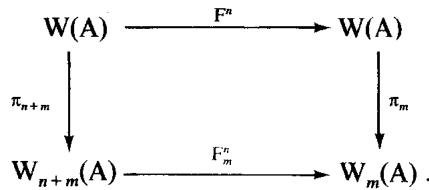
\includegraphics[keepaspectratio]{images/part001_14e9ec0a.jpg}}

回忆（第 3 节），多项式 \(\mathbf{F}_i\) 属于 \(\mathbf{Z}[\mathbf{X}_0, \ldots, \mathbf{X}_{i+1}]\)，对每个整数 \(i \geqslant 0\) 均如此；因此，同态 \(\mathbf{F}_m^1\) 从 \(\mathbf{W}_{m+1}(\mathbf{A})\) 到 \(\mathbf{W}_m(\mathbf{A})\)，可明确写为：

\[
\mathrm{F} _ {m} ^ {1} \left[ a _ {0}, \dots , a _ {m} \right] = \left[ \mathrm{F} _ {i} \left(a _ {0}, \dots , a _ {i + 1}\right) \right] _ {0 \leqslant i <   m}.\tag{46}
\]

设 \(\boldsymbol{a} \in \mathrm{W}_{m}(\mathbf{A})\)、\(\boldsymbol{a}' \in \mathrm{W}_{m}(\mathbf{A})\)，以及 \(\boldsymbol{b} \in \mathrm{W}_{m+1}(\mathbf{A})\)。下列公式由第 5 节命题 3 通过取商得到：

\begin{enumerate}
\def\labelenumi{(\arabic{enumi})}
\setcounter{enumi}{46}
\tightlist
\item
\end{enumerate}

\[
\mathrm{F} _ {m} ^ {1} \left(\mathrm{V} _ {m} ^ {1} (\boldsymbol {a})\right) = p. \boldsymbol {a}\tag{48}
\]

\[
\mathrm{V} _ {m} ^ {1} (a \times \mathrm{F} _ {m} ^ {1} (b)) = \mathrm{V} _ {m} ^ {1} (a) \times b\tag{49}
\]

\[
\mathrm{V} _ {m} ^ {1} (a) \times \mathrm{V} _ {m} ^ {1} (a ^ {\prime}) = p. \mathrm{V} _ {m} ^ {1} (a \times a ^ {\prime})\tag{50}
\]

\[
\mathrm{V} _ {m} ^ {1} (\mathrm{F} _ {m} ^ {1} (b)) = \mu_ {m + 1} \times b
\]

\((\text{其中 } \boldsymbol{\mu}_{m+1} = [0, 1, 0, ..., 0]).\)

